\documentclass[twoside]{ctuthesis}

\usepackage[unicode]{hyperref}
\usepackage{listings}
\usepackage[sorting=none]{biblatex}
\usepackage{todonotes}
\usepackage{array}
\usepackage{textgreek}
\usepackage{float}
\usepackage{multirow}
\usepackage{enumitem}
\usepackage{minted}
\usepackage{verbatim}
\usepackage{xcolor,colortbl}
\usepackage{longtable}
\usepackage{csquotes}

\addbibresource{bibliography/bib_ctu.bib}
\addbibresource{bibliography/bib_research.bib}

\ctusetup{
    author = {Minh Tu Pham},
    supervisor = {Mgr. Ondřej Drbohlav, Ph.D.},
    supervisor-address = {
        Czech Technical University in Prague \\
        Faculty of Electrical Engineering \\
        Department of Cybernetics \\
        Prague, 110 00 \\
        Resslova 307/9 \\
        E-215},
    day = {00},
    year = {2025},
    month = {0},
    title-czech = {Rozpoznávání vizuálních objektů s detekcí neznámých vstupů},
    title-english = {Visual Object Recognition with Unknown Input Detection},
    department-czech = {Katedra kybernetiky},
    department-english = {Department of Cybernetics },
    fieldofstudy-czech = {Otevřená informatika},
    fieldofstudy-english = {Open Informatics},
    subfieldofstudy-czech = {Základy umělé inteligence a počítačových věd},
    subfieldofstudy-english = {Artificial Intelligence and Computer Science},
    keywords-czech = {Detekci mimo distribuci (OOD), Rozpoznávání vizuálních objektů, Vizuální transformátory (ViTs), DINO, Post-hoc metody, Hierarchická detekce, Reprezentace příznaků, Detekce neznámých vstupů},
    keywords-english = {Out-of-Distribution Detection (OOD), Visual Object Recognition, Vision Transformers (ViTs), DINO, Post-Hoc Methods, Hierarchical Detection, Feature Representation, Unknown Input Detection},
    mainlanguage = {english},
    titlelanguage = {english},
    otherlanguages = {czech},
    xfaculty = {F3},
    front-specification = {false},
    pkg-hyperref = false,
    pkg-listings = true,
}

\ctuprocess

\addto\ctucaptionsczech{
	\def\supervisorname{Vedoucí}
	\def\fieldofstudyname{Studijní program}
	\def\subfieldofstudyname{Studijní obor}
}

\setlength{\parskip}{0em}

\begin{abstract-czech}
\\
Tato práce se zabývá klíčovou výzvou detekce vstupů mimo distribuci (OOD) v systémech pro rozpoznávání vizuálních objektů. Ačkoliv výkonné modely, jako jsou konvoluční neuronové sítě (CNN) nebo vizuální transformátory (ViT), dosahují vynikajících výsledků na známých datech, jejich spolehlivost v reálných aplikacích klesá, když se setkají s novými nebo neznámými vstupy.

Tato práce zkoumá různé techniky detekce OOD s využitím bohatých reprezentací příznaků extrahovaných z modelu ViT založeného na DINO.

Náš výzkum má dva hlavní cíle. Prvním je umožnit robustní detekci anomálních vstupů, které leží mimo trénovací data modelu. Druhým je prozkoumat hierarchickou detekci: pokročilejší schopnost, kdy model identifikuje související, avšak nové vstupy tím, že jim přiřadí správnou, širší nadkategorii.

Tato práce hodnotí praktické, post-hoc strategie aplikované na příznaky modelu DINO k dosažení těchto cílů bez náročného přetrénování. Naším cílem je identifikovat efektivní metody, které zlepšují jak odmítání OOD, tak hierarchické chápání, čímž činí tyto vizuální nástroje bezpečnějšími, inteligentnějšími a důvěryhodnějšími pro nasazení v reálném světě.

\end{abstract-czech}

\begin{abstract-english}
\\
This thesis addresses the critical challenge of out-of-distribution (OOD) detection in visual object recognition systems. While powerful models like Convolutional Neural Networks (CNNs) or Vision Transformers (ViTs) perform remarkably well on known data, their reliability in real-world applications diminishes when encountering novel or unknown inputs.

This work explores various OOD detection techniques with rich feature representations extracted from a DINO-based ViT model.

Our research has two primary objectives. First, to enable the robust detection of anomalous inputs that fall outside the model's training data. Second, to explore  hierarchical detection: a more advanced capability where the model identifies related but novel inputs by assigning them to a correct, broader super-category.

This work evaluates practical, post-hoc strategies applied to the DINO model's features to achieve these goals without costly retraining. We aim to identify effective methods that enhance both OOD rejection and hierarchical understanding, thereby making these visual tools safer, more intelligent, and more trustworthy for real-world deployment.
\end{abstract-english}


\begin{document}

\maketitle


\chapter{Introduction}
\label{intro}
Deep learning architectures are currently experiencing a substantial surge in prevalence. Convolutional Neural Networks (CNNs) and Vision Transformers (ViTs) have demonstrated remarkable performance in various computer vision tasks. However, the real world is full of unknowns, which poses serious challenges for these models. When deployed in dynamic environments, they often encounter inputs that differ significantly from their training data, leading to unreliable predictions, \textbf{as illustrated in Figure \ref{fig:yolo_fail}.} The task of identifying such inputs, known as out-of-distribution (OOD) detection, is crucial for ensuring the safety and reliability of AI systems.

\begin{figure}[htbp]
    \centering
    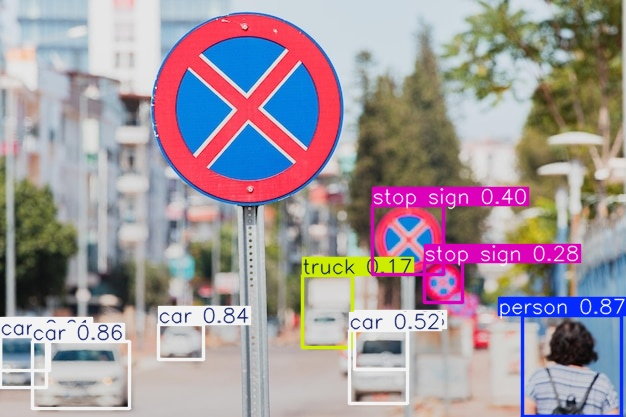
\includegraphics[width=0.9\textwidth]{figures/yolo_sign_failure.jpg}
    \caption[YOLO detection limitations on traffic signs]{Limitations of a standard YOLO detector. The model fails to recognize the nearest `No Parking' sign (False Negative) while misclassifying distant ones as `Stop Signs'. This illustrates the necessity for robust feature representations.}
    \label{fig:yolo_fail}
\end{figure}

Previous research has primarily focused on binary OOD detection, where models must distinguish only between in-distribution (ID) and OOD samples.\cite{wallin2025prohocprobabilistichierarchicaloutofdistribution}
While this is an important step towards robust AI, it does not fully capture the complexity of real-world scenarios. For example, when an autonomous vehicle encounters an unseen input, it is insufficient to simply flag it as OOD. Instead, a hierarchical approach assigns it to a generic class (e.g., `obstacle'), preserving semantic information essential for decision-making.

To address these challenges, this thesis explores the capabilities of self-supervised Vision Transformers, specifically the DINOv3 architecture\cite{siméoni2025dinov3}. We selected this model for its state-of-the-art performance on out-of-distribution benchmarks (as shown in ObjectNet evaluations) and its ability to produce rich semantic representations while being kept frozen. This "frozen" capability allows for substantial computational savings, making the model ideal for efficient \textbf{post-hoc} analysis without the need for extensive fine-tuning.

\section{Contributions}
\label{intro_sekce}
The following sections summarize the main contributions of this thesis:

\begin{enumerate}
    \item
    \item
    \item
\end{enumerate}


\chapter{Related Work}
\label{related_work}
This chapter reviews the existing literature relevant to the thesis. It covers the evolution of visual backbone architectures focused on Vision Transformers and Self-Supervised Learning. 
In due course, it delves into established methodologies for OOD detection. 
Finally, it explores the emerging concept of hierarchical OOD detection, highlighting its significance and the challenges it presents.

\section{Visual Representation Learning}
\label{sec:rel_representation}
State-of-the-art computer vision architectures have evolved significantly from traditonal CNNs to more sophisticated models like ViTs.

\subsection{Vision Transformers (ViT)}
\label{sec:rel_vit}
Vision Transformers (ViTs)\cite{dosovitskiy2021imageworth16x16words} have revolutionized and dethroned CNNs as the dominant architecture in computer vision. 
Unlike CNNs, which process images via local receptive fields and convolutional layers, ViTs leverage the self-attention mechanism from the Transformer architecture\cite{vaswani2023attentionneed} to capture global dependencies in images.

\subsection{Self-Supervised Learning and DINO}
\label{sec:rel_ssl_dino}
Training ViTs typically requires massive labeled datasets. To mitigate this, Self-Supervised Learning (SSL) has emerged as a powerful alternative. Methods like DINO (Distillation with No Labels) \cite{caron2021emergingpropertiesselfsupervisedvision} and its successors, DINOv2 and DINOv3 \cite{siméoni2025dinov3}, learn robust features by enforcing consistency between different views of the same image.

\section{Out-of-Distribution Detection}
\label{sec:rel_ood}

\printbibliography[title=Literature]

\appendix

\chapter{List of Abbreviations}
\label{app_shortcuts}

\begin{center}
    \begin{tabular}{r p{25em}}
        \textbf{ViT}             &  Vision Transformer \\
        \textbf{CNN}             &   Convolutional Neural Network \\
        \textbf{OOD}             &   Out-of-Distribution \\
        \textbf{DINO}            &   Self-Distillation with No Labels \\
        \textbf{ID}             &   In-Distribution \\
        \textbf{SSL}            &   Self-Supervised Learning \\
    \end{tabular}
\end{center}


\end{document}
